\section{Semantics}

\begin{frame}
    \frametitle{We need some meaning}

    \pause
    Values are interpreted in a \alert{lattice}:

    \pause
    \begin{minipage}{0.49\textwidth}
        \[
            \scalebox{1.5}{\tikzfig{circuits/a4}}
        \]
    \end{minipage}
    \pause
    \begin{minipage}{0.49\textwidth}
        \begin{align*}
            \dsptikzfig{strings/structure/monoid/init}[colour=comb]
            \,&\mapsto\, \bot \\
            \dsptikzfig{circuits/components/values/vs}[val=\belnapfalse]
            \,&\mapsto\, 0 \\
            \dsptikzfig{circuits/components/values/vs}[val=\belnaptrue]
            \,&\mapsto\, 1 \\
            \dsptikzfig{circuits/components/values/vs}[val=\belnapboth]
            \,&\mapsto\, \top
        \end{align*}
    \end{minipage}
\end{frame}
\begin{frame}
    \frametitle{Let's make everything a function}

    \pause
    \setlength{\tabcolsep}{1.5em}
    \renewcommand{\arraystretch}{2}

    \begin{center}
        \begin{tabular}{lrl}
            \dsptikzfig{circuits/components/gates/gate}[gate=g]
            &
            \alert{monotone functions}
            &
            \(\morph{\overline{g}}{\valuetuple{m}}{\values}\)
            \\
            \pause
            \hspace{0.175cm}
            \dsptikzfig{strings/structure/monoid/init}[colour=comb]
            &
            \alert{initialise}
            &
            \(() \mapsto (\bot)\)
            \\
            \pause
            \dsptikzfig{strings/structure/comonoid/copy}[colour=comb]
            &
            \alert{copy}
            &
            \(x \mapsto (x, x)\)
            \\
            \pause
            \dsptikzfig{strings/structure/monoid/merge}[colour=comb]
            &
            \alert{join in the lattice}
            &
            \((x, y) \mapsto x \ljoin y\)
            \\
            \pause
            \dsptikzfig{strings/structure/comonoid/discard}[colour=comb]
            &
            \alert{discard}
            &
            \(x \mapsto ()\)
        \end{tabular}
        \pause

        \vspace{0.5em}

        Feedback is interpreted as the \alert{least fixed point}.
    \end{center}
\end{frame}
\begin{frame}
        \frametitle{Functions are not enough}

        \centering
        \LARGE
        How do we model \alert{delay}?

        \pause
        \alert{Streams!}
\end{frame}
\begin{frame}
    \frametitle{Streams}

    A \alert{stream} \(\stream{\values}\) is an infinite sequence of values.
    \[
        v_0
        \streamcons
        v_1
        \streamcons
        v_2
        \streamcons
        v_3
        \streamcons
        v_4
        \streamcons
        v_5
        \streamcons
        v_6
        \streamcons
        v_7
        \streamcons
        \cdots
    \]

    \pause
    A \alert{stream function} \(\stream{\values} \to \stream{\values}\) consumes and
    produces streams.
    \[
        f(
            v_0
            \streamcons
            v_1
            \streamcons
            v_2
            \streamcons
            v_3
            \streamcons
            v_4
            \streamcons
            \cdots
        ) =
        w_0
        \streamcons
        w_1
        \streamcons
        w_2
        \streamcons
        w_3
        \streamcons
        w_4
        \streamcons
        \cdots
    \]
\end{frame}
\begin{frame}
    \frametitle{Interpreting the sequential components}

    \LARGE

    \pause
    \[
        \dsptikzfig{circuits/components/values/vs}[val=v]()
        :=
        v \streamcons \bot \streamcons \bot \streamcons \bot \streamcons \cdots
    \]

    \pause
    \vspace{0.5em}

    \[
        \normalsize
        \dsptikzfig{circuits/components/waveforms/delay}
        \LARGE(
            v_0 \streamcons v_1 \streamcons v_2 \streamcons \cdots
        )
        :=
        \bot \streamcons v_0 \streamcons v_1 \streamcons v_2 \streamcons \cdots
    \]
\end{frame}
\begin{frame}{Maybe there are too many streams}

    \centering
    \LARGE
    Does every circuit correspond to a stream function \(
        \valuetuplestream{m} \to \valuetuplestream{n}
    \)?

    \Huge
    \pause
    No.

    \scriptsize
    \pause
    (but this is to be expected!)
\end{frame}
\begin{frame}
    \frametitle{Restricting the stream functions}

    \pause
    \Large
    Circuits are \alert{causal}.

    \pause

    \normalsize
    They can only depend \alert{what they've seen so far}.

    \pause

    \Large
    Circuits are \alert{monotone}.

    \pause

    \normalsize
    They are constructed from \alert{monotone functions}.

    \pause

    Is that all?
    \pause
    \alert{Not quite...}
    \pause
    (but we'll get there)


\end{frame}
\begin{frame}
    \frametitle{Some operations on stream functions}

    Given a causal stream function \(
        \morph{f}{\valuetuplestream{m}}{\valuetuplestream{n}}
    \) and an element \(a \in \valuetuple{m}\)...

    \pause

    \Large
    \alert{initial output} \quad
    \(\mealyoutput{f}{a} \in \valuetuple{n}\)

    \pause

    \normalsize
    `the first thing \(f\) produces given \(a\)'

    \pause

    \Large
    \alert{stream derivative} \quad
    \(\mealytransition{f}{a} \in \valuetuplestream{m} \to \valuetuplestream{n}\)

    \pause

    \normalsize
    `how \(f\) behaves after seeing \(a\) first'

    \vspace{1em}

    \pause
    Hold on, these look familiar...

\end{frame}
\begin{frame}
    \frametitle{An old friend}

    \Large

    \begin{center}
        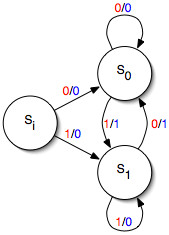
\includegraphics[scale=0.5]{imgs/mealy-machine}

        Mealy machines!

        \pause

        \normalsize
        Stream functions are the \emph{states} in a Mealy machine.
    \end{center}

\end{frame}
\begin{frame}
    \frametitle{Circuits have finitely many behaviours}

    Circuits have a finite number of components.

    \pause

    So there are finite number of states in the Mealy machine.

    \pause

    So the outputs of streams given some input must be \alert{periodic}.

    \pause

    (There are finitely many \alert{stream derivatives}).
\end{frame}
\begin{frame}
    \frametitle{These are the streams we're looking for}

    \begin{theorem}
        A stream function is the interpretation of a sequential circuit
        if and only if it is \textbf{causal}, \textbf{monotone} and has
        \textbf{finitely many stream derivatives}.
    \end{theorem}
\end{frame}
\begin{frame}
    \frametitle{The correspondence}

    \centering
    \Large

    \begin{tikzcd}[ampersand replacement=\&,row sep=large]
        \&
        \text{Circuits}
        \arrow[visible on=<2->]{dl}
        \arrow[visible on=<3->]{dr}
        \&
        \\
        \text{Stream functions}
        \arrow[visible on=<5->,bend left]{ur}
        \arrow[visible on=<4->]{rr}
        \&
        \&
        \text{Mealy machines}
        \arrow[visible on=<5->,bend right]{ul}
        \arrow[visible on=<4->,bend left]{ll}
    \end{tikzcd}
\end{frame}